\section{Análise preliminar}

Na análise preliminar, utiliza-se LTSPICE em adição à análise de circuitos e parâmetros h para encontrar analiticamente os valores de \emph{A, $A_f$, $\beta$, $R_i$, $R_{if}$, $R_o$ e $R_{o f}$}.

\begin{figure}[h]
    \centering
    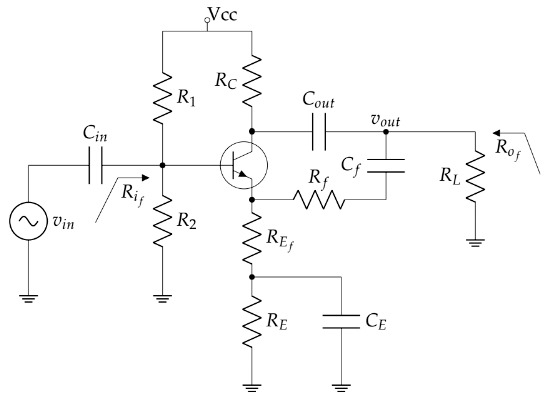
\includegraphics[width=0.5\columnwidth]{Images/o_circuito.png}
    \caption{Circuito em análise.}
\end{figure}

\subsection{$A_f$}

Monta-se o circuito no LTSpice e faz-se que $A_f = \frac{V_o}{V_i}$. O que nos dá $A_f \approx 4.06$.

\begin{figure}[h]
    \centering
    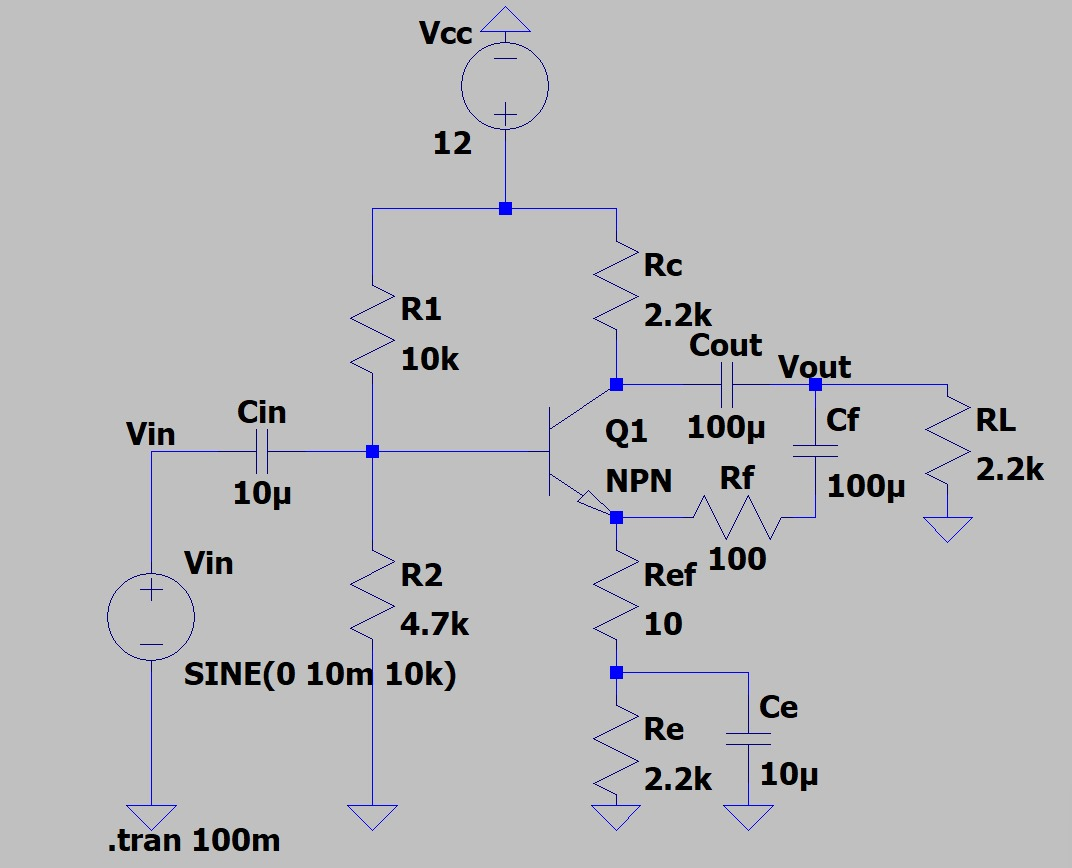
\includegraphics[width=0.5\columnwidth]{Images/circuito_ltspice.jpeg}
    \caption{Circuito no LTSpice.}
\end{figure}

\begin{figure}[h]
    \centering
    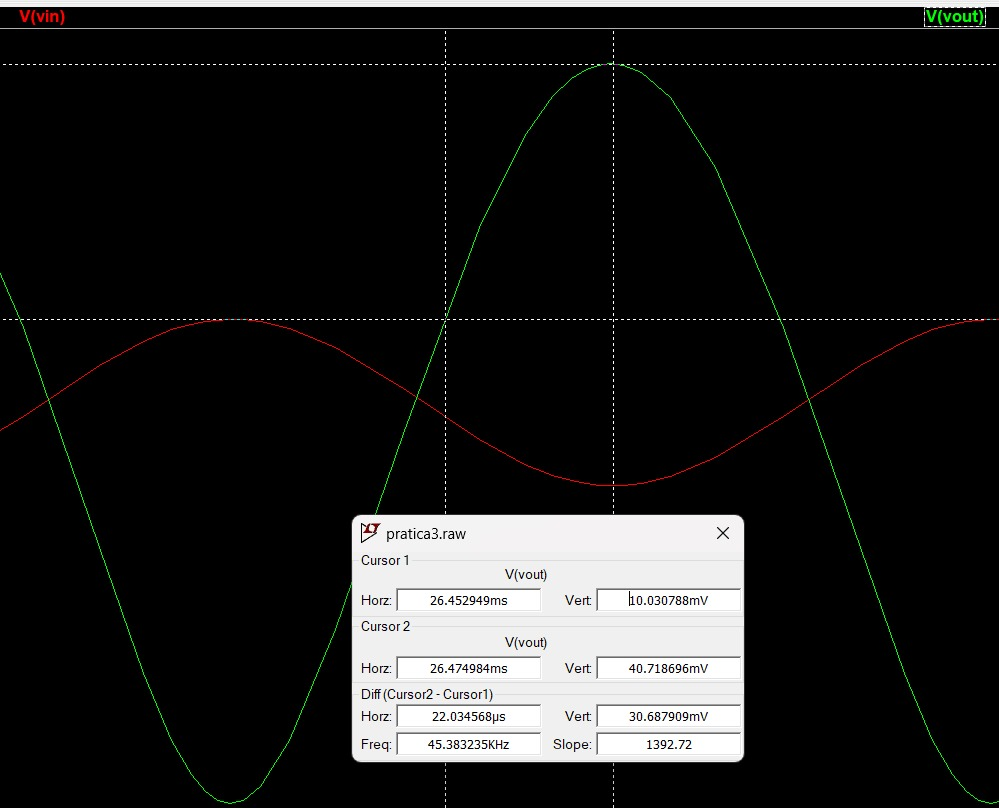
\includegraphics[width=0.8\columnwidth]{Images/circuito_ltspice_ganho.jpeg}
    \caption{Ganho do circuito no LTSpice.}
\end{figure}

\subsection{$\beta$}

Faz-se cálculo do parâmetro $h_{12}$ para encontrar o $\beta$ da seguinte maneira:

\begin{equation}
    \begin{aligned}
         & \beta = h_{12} = \frac{V_1}{V_2} | I_1 = 0                                    \\
         & \beta = \frac{R_1 i_2}{\left( R_1 + R_2 \right) i_2} = \frac{10}{110} = 0.091
    \end{aligned}
\end{equation}

\begin{figure}[h]
    \centering
    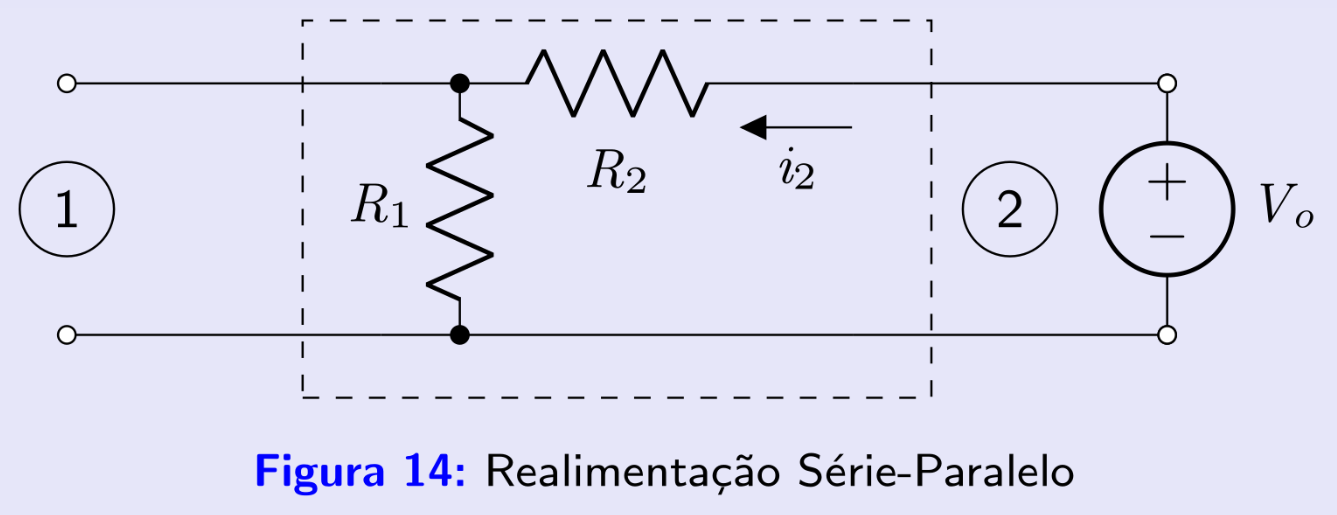
\includegraphics[width=0.5\columnwidth]{Images/realimentacao_beta.png}
    \caption{Circuito de realimentação.}
\end{figure}

\subsection{$A$}

Tem-se a seguinte relação entre $A$ e o $A_f$ e $\beta$ previamente calculados:

\begin{equation}
    \begin{aligned}
         & A_f = \frac{A}{1 + A\beta}                  \\
         & A = \frac{A_f}{1 - A_f \beta} \approx 6.435
    \end{aligned}
\end{equation}

\subsection{$R_i$ e $R_o$}

Primeiro precisa-se calcular os valores de $R_{11}$ e $R_{22}$. E analisando o circuito como um quadripolo tem-se:

\begin{equation}
    \begin{aligned}
        R_{11} = R_{Ef} // R_f \approx 9.09 \varOmega \\
        R_{22} = R_{Ef} + R_f = \approx 110 \varOmega
    \end{aligned}
\end{equation}

Com estes em mãos, pode-se adicionar o $R_{11}$ em série na entrada e o $R_{22}$ em paralelo na saída.

Acha-se valores de $I_c$ pelo LTSPice, e $hFE$ no site: \url{https://www.digikey.com/en/products/detail/microchip-technology/2N2222AUB/4377384?utm_source=findchips&utm_medium=aggregator&utm_campaign=buynow}

\begin{equation}
    \begin{aligned}
         & I_c \approx 1.35mA                                              \\
         & gm = \frac{I_c}{V_t} \approx 0.054S                             \\
         & hFE = 100                                                       \\
         & R_{\pi} = \frac{hFE}{gm} \approx 1851.85 \varOmega              \\
         & R_i = R_1 // R_2 // (R_{11} + R_{\pi}) \approx 1172.7 \varOmega \\
         & R_o = R_C // R_L // R_{22} = 100 \varOmega
    \end{aligned}
\end{equation}

\subsection{$R_{if}$ e $R_{of}$}

Com os valores das resistências de entrada e de saída em mãos, pode-se achar $R_{if}$ e $R_{of}$:

\begin{equation}
    \begin{aligned}
         & R_{if} = R_i (1 + A \beta) = 1858.75 \varOmega     \\
         & R_{of} = \frac{R_o}{1 + A \beta} = 63.09 \varOmega
    \end{aligned}
\end{equation}

\subsection{Frequências de corte}

Analisando o gráfico de Bode no LTSpice, identificam-se informações cruciais para compreender o comportamento do sistema em diferentes frequências.

\begin{figure}[h]
    \centering
    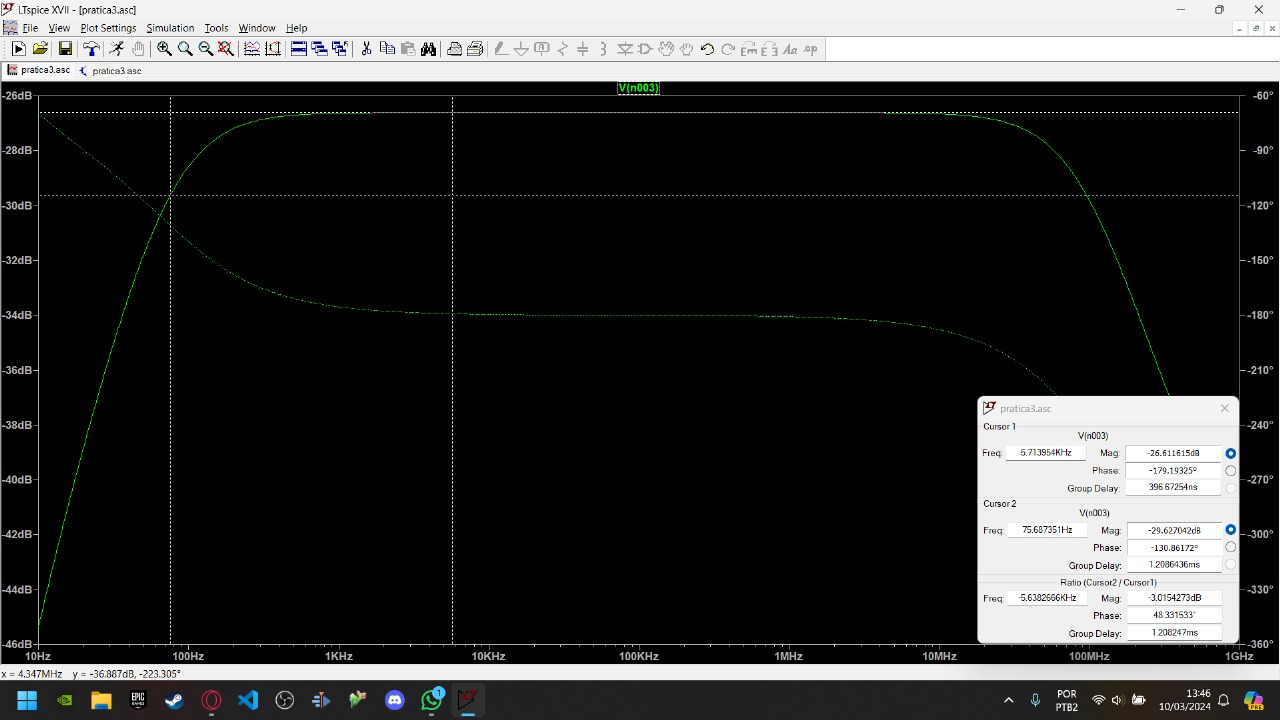
\includegraphics[width=0.8\columnwidth]{Images/fc.jpeg}
    \caption{Obtendo a $F_c$ do grafico de Bode no LTSpice.}
\end{figure}

\begin{figure}[h]
    \centering
    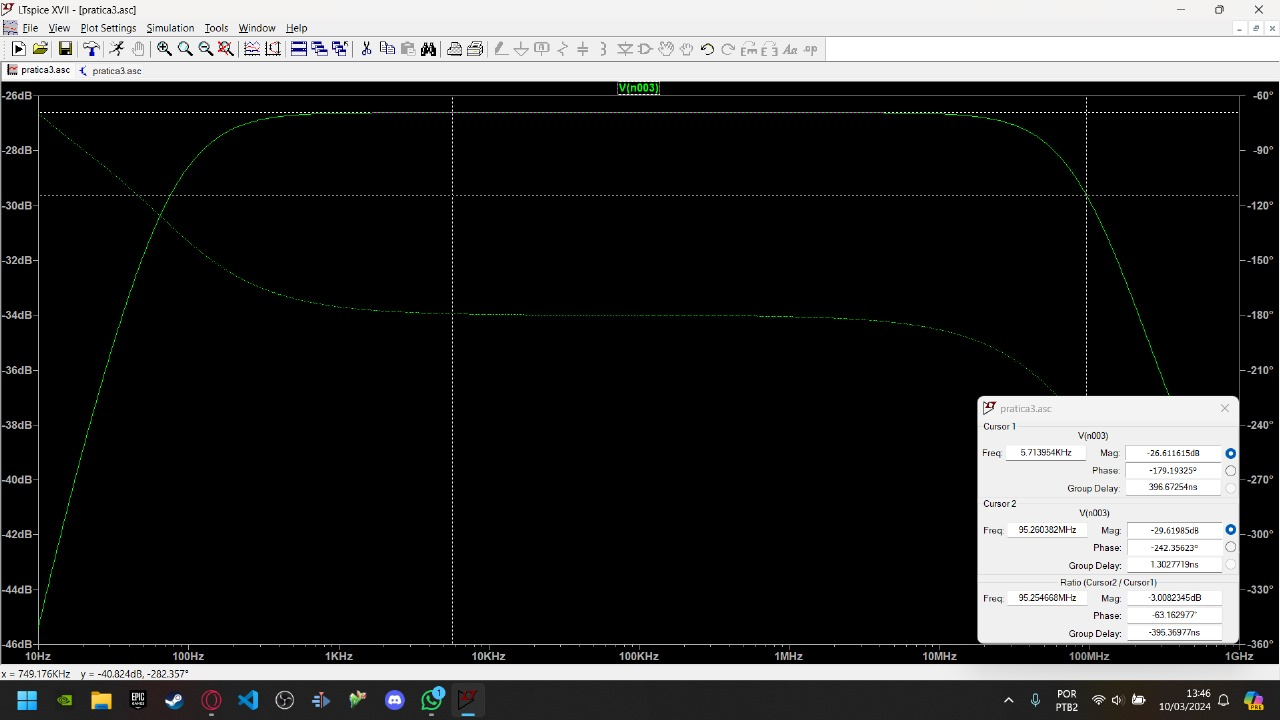
\includegraphics[width=0.8\columnwidth]{Images/fh.jpeg}
    \caption{Obtendo a $F_h$ do grafico de Bode no LTSpice.}
\end{figure}
